\documentclass[8pt]{extarticle}
\title{}
\author{Avinash Iyer}
\date{}
\usepackage[shortlabels]{enumitem}

%font setup
%
%\usepackage[math]{anttor}

%paper setup
\usepackage{geometry}
\geometry{letterpaper, portrait, margin=1in}
\usepackage{fancyhdr}

%symbols
\usepackage{amsmath}
\usepackage{amssymb}
\usepackage{hyperref}
\usepackage{gensymb}

\usepackage[T1]{fontenc}
\usepackage[utf8]{inputenc}

%chemistry stuff
\usepackage[version=4]{mhchem}
\usepackage{chemfig}

%plotting
\usepackage{pgfplots}
\usepackage{tikz}

%\usepackage{natbib}

%graphics stuff
\usepackage{graphicx}
\graphicspath{ {./images/} }

%code stuff
%when using minted, make sure to add the -shell-escape flag
%you can use lstlisting if you don't want to use minted
%\usepackage{minted}
%\usemintedstyle{pastie}
%\newminted[javacode]{java}{frame=lines,framesep=2mm,linenos=true,fontsize=\footnotesize,tabsize=3,autogobble,}
%\newminted[cppcode]{cpp}{frame=lines,framesep=2mm,linenos=true,fontsize=\footnotesize,tabsize=3,autogobble,}

\usepackage{listings}
\usepackage{color}
\definecolor{dkgreen}{rgb}{0,0.6,0}
\definecolor{gray}{rgb}{0.5,0.5,0.5}
\definecolor{mauve}{rgb}{0.58,0,0.82}

\lstset{frame=tb,
	language=Java,
	aboveskip=3mm,
	belowskip=3mm,
	showstringspaces=false,
	columns=flexible,
	basicstyle={\small\ttfamily},
	numbers=none,
	numberstyle=\tiny\color{gray},
	keywordstyle=\color{blue},
	commentstyle=\color{dkgreen},
	stringstyle=\color{mauve},
	breaklines=true,
	breakatwhitespace=true,
	tabsize=3
}
% text + color boxes
\usepackage{tcolorbox}
\tcbuselibrary{breakable}
\newtcolorbox{problem}[1]{colback = white, colframe = black, title = {#1}}
\newtcolorbox{solution}{colback = white, title = Solution, breakable}
%including PDF
\usepackage{pdfpages}
\setlength{\parindent}{0pt}

\pagestyle{fancy}
\fancyhf{}
\rhead{Avinash Iyer}
\lhead{Problem Set 3}
\begin{document}
\begin{problem}{South Korea vs. Philippines}
  In 1960, South Korea and the Philippines had similar economic characteristics, in terms of per capita GDP (\~\$1500), population (25 million, $1/2$ working age), similar sectoral composition (industry, agriculture), and college enrollment (Korea = 5\%, Philippines = 13\%). Yet, after 1960, macroeconomic performance diverged sharply. By 2017, per capita GDP in Korea was about \$36000, roughly two thirds the U.S. Level. Meanwhile, per capita GDP in the Philippines was only \$7700.
  \begin{enumerate}[(a)]
    \item The graph below displays the investment rate in South Korea, the Philippines, and the United States between 1960 and 2017. Is the higher level of GDP per capita in South Korea relative to the Philippines consistent with the predictions of the Solow Growth Model? Illustrate with a Solow diagram.
    \item As shown below, the investment rate in the Philippines is roughly the same as the investment rate in the United States. Yet, GDP per capita in the United States is roughly seven times higher than in the Philippines. Assuming that the rate of depreciation of capital is the same in both countries, according to the Solow Model, what variable must account for the higher per capita income level in the U.S.? Can you assign a numerical estimate to your answer? How much higher is this variable in the U.S. than in the Philippines?
    \item Parts (a) and (b) illustrate the strengths and weaknesses of the Solow Model, as described in section 5.10 of the textbook. What are those strengths and weaknesses? Explain.
  \begin{center}
    \includegraphics[width=10cm]{ps3_img1}          
  \end{center}
  \end{enumerate}
\end{problem}
\begin{solution}
  \begin{tcolorbox}[colframe = black!75!white, title = (a), colback = white]
      The higher level of per capita GDP in South Korea is consistent with the Solow Growth model as it predicts a higher level of capital accumulation before steady state is reached. A rudimentary illustration is shown below:
      \begin{center}
        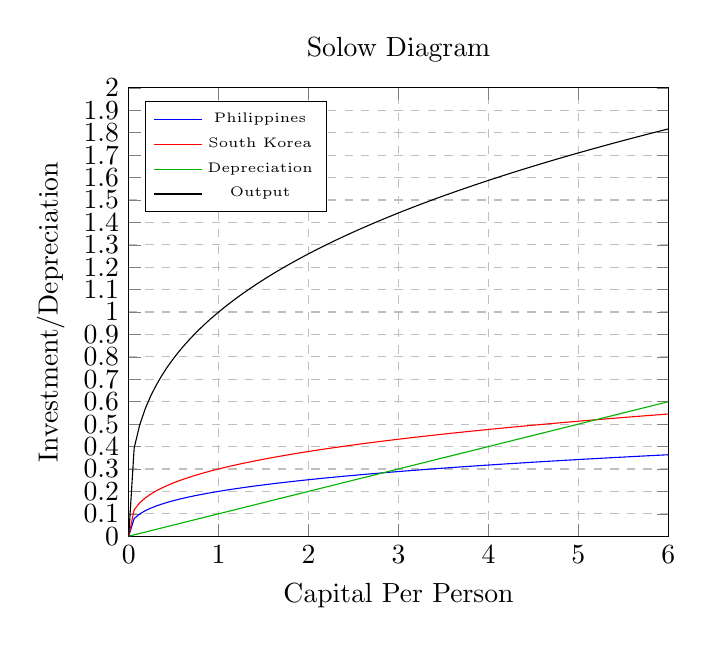
\begin{tikzpicture}
          \begin{axis}[
              title = {Solow Diagram},
              ylabel = {Investment/Depreciation},
            xlabel = {Capital Per Person},
          xmin = 0, xmax = 6,
          ymin = 0, ymax = 2,
          xtick = {0,1,2,3,4,5,6},
          ytick = {0,0.1,0.2,0.3,0.4,0.5,0.6,0.7,0.8,0.9,1.0,1.1,1.2,1.3,1.4,1.5,1.6,1.7,1.8,1.9,2.0},
          legend pos = north west,
          xmajorgrids = true, ymajorgrids = true, grid style = dashed,
        ]
        \addplot[color = blue, samples = 100, domain = 0:6]{0.2*x^(1/3)};
        \addlegendentry{\tiny Philippines}
        \addplot[color = red, samples = 100, domain = 0:6]{0.3*x^(1/3)};
        \addlegendentry{\tiny South Korea}
        \addplot[color = green!70!black, samples = 100, domain = 0:6]{0.1*x};
        \addlegendentry{\tiny Depreciation}
        \addplot[color = black, samples = 100, domain = 0:6]{x^(1/3)};
        \addlegendentry{\tiny Output}
      \end{axis}
    \end{tikzpicture}
  \end{center}
  As we can see above, the rate at which depreciation and investment are equivalized would be higher in Korea (with about a 30\% investment rate) than in the Philippines (with about a 20\% investment rate). This means that output will be higher in South Korea than in the Philippines. 
\end{tcolorbox} 
  \begin{tcolorbox}[colframe = black!75!white, title = (b), colback = white]
    Though the investment rate in the United States and the Philippines are about the same, the main reason the United States has roughly 7 times the GDP per capita as the Philippines is because the United States has a higher Total Factor Productivity, or $\overline{A}$, which we can roughly estimate to be about $7$.
  \end{tcolorbox}
  \begin{tcolorbox}[colframe = black!75!white, title = (c), colback = white]
    The Solow Model is particularly good at explaining the differences between countries with similar economic starting points but different rates of capital accumulation, and shows how differing rates of investment will change the eventual capital per person in the economy.\\

    The main drawback of the Solow Model is that it does not model changes in Total Factor Productivity, which are the overwhelming differences between different countries' output per capita.
  \end{tcolorbox}
\end{solution}
\begin{problem}{An Increase in Total Factor Productivity}
  Suppose that the level of TFP in an economy rises from $\overline{A}$ to $\overline{A}'$.
  \begin{enumerate}[(a)]
    \item Assuming the economy starts from its initial steady state, use the Solow model to explain what happens to the economy over time. 
    \item Draw a graph showing how output evolves over time.
    \item Suppose that $\overline{A}$ grew at a constant rate, instead of being constant. Explain in words what you think would happen to GDP over time.
  \end{enumerate}
\end{problem}
\begin{solution}
  \begin{tcolorbox}[colframe = black!75!white, title = (a), colback = white]
    Both output and investment increase as TFP pulls the rate of capital accumulation above depreciation --- as depreciation catches up, the rate of output growth slows until we reach a new equilibrium.
  \end{tcolorbox}
  \begin{tcolorbox}[title = (b), colback = white, breakable]
      \begin{center}
        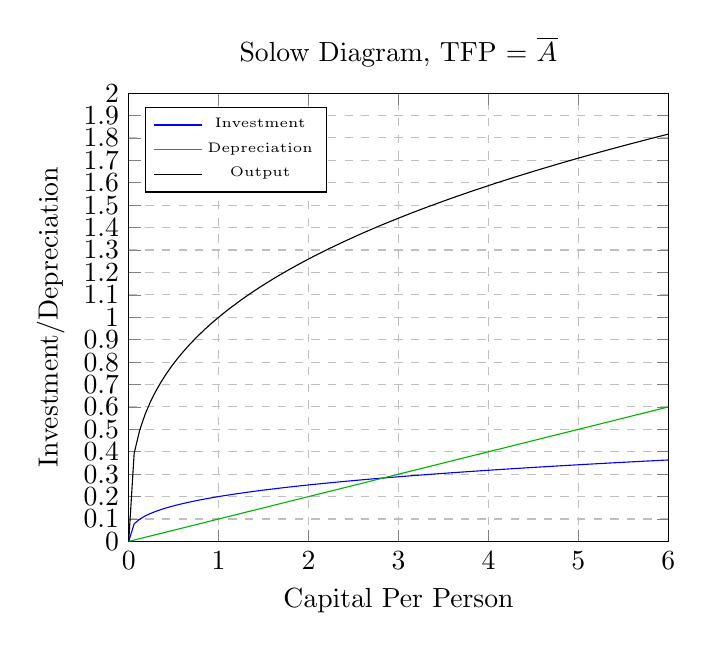
\begin{tikzpicture}
          \begin{axis}[
            title = {Solow Diagram, TFP = $\overline{A}$},
              ylabel = {Investment/Depreciation},
            xlabel = {Capital Per Person},
          xmin = 0, xmax = 6,
          ymin = 0, ymax = 2,
          xtick = {0,1,2,3,4,5,6},
          ytick = {0,0.1,0.2,0.3,0.4,0.5,0.6,0.7,0.8,0.9,1.0,1.1,1.2,1.3,1.4,1.5,1.6,1.7,1.8,1.9,2.0},
          legend pos = north west,
          xmajorgrids = true, ymajorgrids = true, grid style = dashed,
        ]
        \addplot[color = blue, samples = 100, domain = 0:6]{0.2*x^(1/3)};
        \addlegendentry{\tiny Investment}
        \addplot[color = green!70!black, samples = 100, domain = 0:6]{0.1*x};
        \addlegendentry{\tiny Depreciation}
        \addplot[color = black, samples = 100, domain = 0:6]{x^(1/3)};
        \addlegendentry{\tiny Output}
      \end{axis}
    \end{tikzpicture}\\
    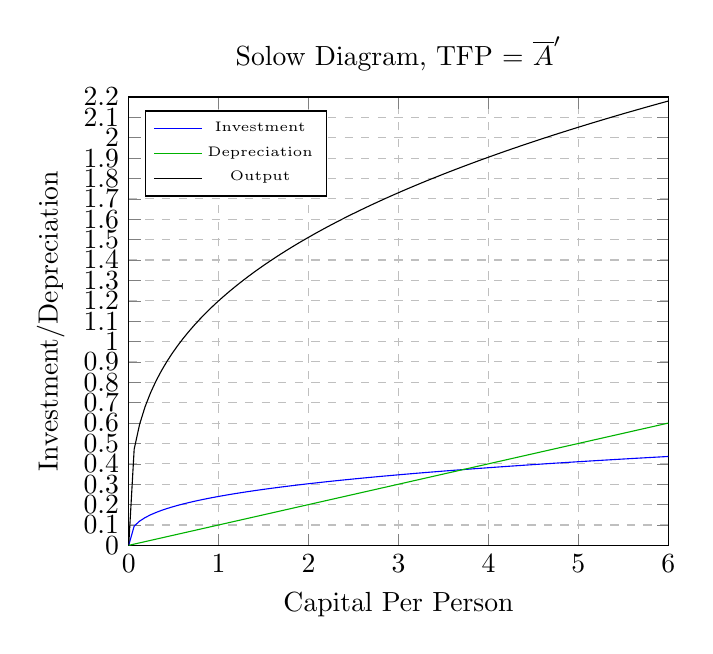
\begin{tikzpicture}
          \begin{axis}[
            title = {Solow Diagram, TFP = $\overline{A}'$},
              ylabel = {Investment/Depreciation},
            xlabel = {Capital Per Person},
          xmin = 0, xmax = 6,
          ymin = 0, ymax = 2.2,
          xtick = {0,1,2,3,4,5,6},
          ytick = {0,0.1,0.2,0.3,0.4,0.5,0.6,0.7,0.8,0.9,1.0,1.1,1.2,1.3,1.4,1.5,1.6,1.7,1.8,1.9,2.0,2.1,2.2},
          legend pos = north west,
          xmajorgrids = true, ymajorgrids = true, grid style = dashed,
        ]
        \addplot[color = blue, samples = 100, domain = 0:6]{1.2 * 0.2*x^(1/3)};
        \addlegendentry{\tiny Investment}
        \addplot[color = green!70!black, samples = 100, domain = 0:6]{0.1*x};
        \addlegendentry{\tiny Depreciation}
        \addplot[color = black, samples = 100, domain = 0:6]{1.2 * x^(1/3)};
        \addlegendentry{\tiny Output}
      \end{axis}
    \end{tikzpicture}
  \end{center}
  \end{tcolorbox}
  \begin{tcolorbox}[title = (c), colback = white, breakable]
    If $\overline{A}$ grew at a constant rate instead of being constant, GDP over time would tend to increase at a rate of $\overline{A}^{3/2}$, which is the exponent in the Solow model, since at every point in time, steady state grows to require increased output, meaning that GDP will reach steady state at an increasing level of output.
  \end{tcolorbox}
\end{solution}
\begin{problem}{Per capita GDP in the Long Run}
  Suppose an economy begins in steady state. According to the Solow Growth Model, by what proportion does per capita GDP change in the long run in response to each of the following changes:
  \begin{enumerate}[(a)]
    \item The investment rate doubles.
    \item The depreciation rate falls by 10\%.
    \item The productivity level rises by 10\%
  \end{enumerate}
\end{problem}
\begin{solution}
  \begin{tcolorbox}[title = (a), colback = white, breakable]
    \begin{align*}
      y^{*} &= \overline{A}^{3/2}\left(\frac{\overline{s}}{\overline{d}}\right)^{1/2}\\
      y^{**} &= \overline{A}^{3/2}\left(\frac{\overline{s}'}{\overline{d}}\right)^{1/2}\\
             &= 1.41y^{*}
    \end{align*}
  \end{tcolorbox}
  \begin{tcolorbox}[colback = white, title = (b)]
    \begin{align*}
      y^{*} &= \overline{A}^{3/2}\left(\frac{\overline{s}}{\overline{d}}\right)^{1/2}\\
      y^{**} &= \overline{A}^{3/2}\left(\frac{\overline{s}}{0.9\overline{d}}\right)^{1/2}\\
           &= 1.05 y^*
    \end{align*}
  \end{tcolorbox}
  \begin{tcolorbox}[colback = white, title = (c)]
    \begin{align*}
      y^{*} &= \overline{A}^{3/2}\left(\frac{\overline{s}}{\overline{d}}\right)^{1/2}\\
      y^{**} &= 1.1\overline{A}^{3/2}\left(\frac{\overline{s}}{\overline{d}}\right)^{1/2}\\
             &= 1.15y^*
    \end{align*}
  \end{tcolorbox}
\end{solution}
\begin{problem}{A variation of the Solow Model}
  This problem studies a Solow economy where the fraction of the population that works, $\overline{x}$ is allowed to be different from $1$. This is the setup:
  \begin{align*}
    Y_t &= \overline{A}K_t^{1/3}L_t^{2/3}\\
    \Delta K_t &= I_t - \overline{d}K_t, K_0 = \overline{K}_0\\
    C_t + I_t &= Y_t \\
    I_t &= \overline{s}Y_t \\
    L_t &= \overline{x}\overline{N}
  \end{align*}
  \begin{enumerate}[(a)]
    \item What are the endogenous variables in this problem? What are the exogenous parameters?
    \item Suppose the economy begins at steady state. Then, the fraction of the population that works immediately and permanently rises to $\overline{x}'$. Using a Solow diagram, explain how the capital stock evolves over time.
    \item Solve algebraically for the new steady state level of output.
    \item Draw a graph showing how per capita output evolves over time.
  \end{enumerate}
\end{problem}
\begin{solution}
  \begin{tcolorbox}[colback = white, title = (a)]
    The endogenous variables are as follows:
    \begin{itemize}
      \item $K_t$
      \item $Y_t = \overline{A}K_t^{1/3}\left(\overline{x}\overline{N}\right)^{2/3}$
      \item $I_t$
    \end{itemize}
    The exogenous parameters are as follows:
    \begin{itemize}
      \item $\overline{s}$
      \item $\overline{d}$
      \item $\overline{x}$
      \item $\overline{N}$
      \item $\overline{K}_0$
      \item $\overline{A}$
    \end{itemize}
  \end{tcolorbox}
  \begin{tcolorbox}[colback = white, title = (b)]
    \begin{center}
      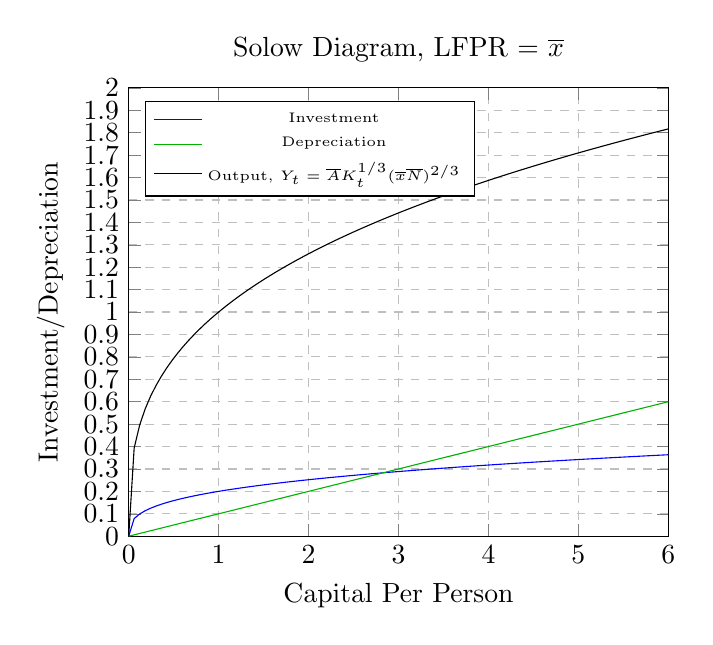
\begin{tikzpicture}
        \begin{axis}[
          title = {Solow Diagram, LFPR = $\overline{x}$},
            ylabel = {Investment/Depreciation},
          xlabel = {Capital Per Person},
        xmin = 0, xmax = 6,
        ymin = 0, ymax = 2,
        xtick = {0,1,2,3,4,5,6},
        ytick = {0,0.1,0.2,0.3,0.4,0.5,0.6,0.7,0.8,0.9,1.0,1.1,1.2,1.3,1.4,1.5,1.6,1.7,1.8,1.9,2.0},
        legend pos = north west,
        xmajorgrids = true, ymajorgrids = true, grid style = dashed,
      ]
      \addplot[color = blue, samples = 100, domain = 0:6]{0.2*x^(1/3)};
      \addlegendentry{\tiny Investment}
      \addplot[color = green!70!black, samples = 100, domain = 0:6]{0.1*x};
      \addlegendentry{\tiny Depreciation}
      \addplot[color = black, samples = 100, domain = 0:6]{x^(1/3)};
      \addlegendentry{\tiny Output, $Y_t = \overline{A}K_t^{1/3}(\overline{x}\overline{N})^{2/3}$}
    \end{axis}
  \end{tikzpicture}\\
  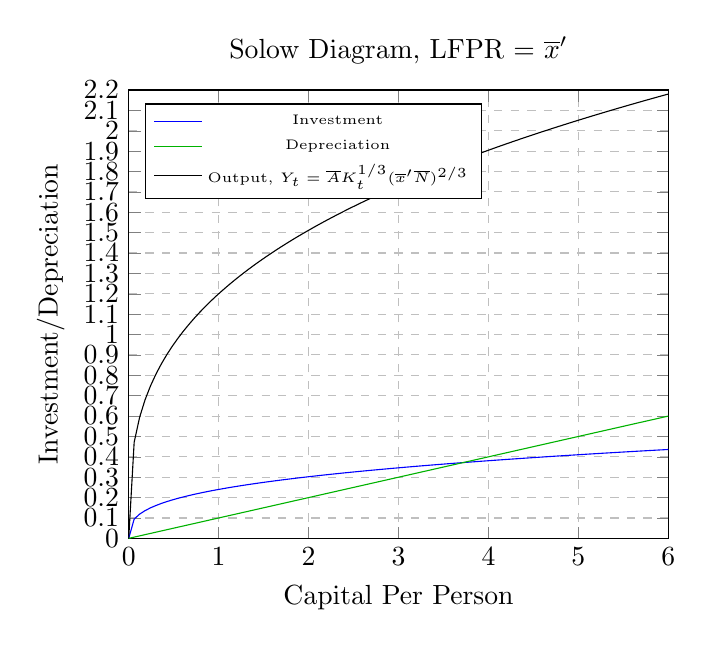
\begin{tikzpicture}
        \begin{axis}[
          title = {Solow Diagram, LFPR = $\overline{x}'$},
          ylabel = {Investment/Depreciation},
          xlabel = {Capital Per Person},
          xmin = 0, xmax = 6,
          ymin = 0, ymax = 2.2,
          xtick = {0,1,2,3,4,5,6},
          ytick = {0,0.1,0.2,0.3,0.4,0.5,0.6,0.7,0.8,0.9,1.0,1.1,1.2,1.3,1.4,1.5,1.6,1.7,1.8,1.9,2.0,2.1,2.2},
          legend pos = north west,
          xmajorgrids = true, ymajorgrids = true, grid style = dashed,
      ]
      \addplot[color = blue, samples = 100, domain = 0:6]{1.2 * 0.2*x^(1/3)};
      \addlegendentry{\tiny Investment}
      \addplot[color = green!70!black, samples = 100, domain = 0:6]{0.1*x};
      \addlegendentry{\tiny Depreciation}
      \addplot[color = black, samples = 100, domain = 0:6]{1.2 * x^(1/3)};
      \addlegendentry{\tiny Output, $Y_t = \overline{A}K_t^{1/3}(\overline{x}'\overline{N})^{2/3}$}
    \end{axis}
  \end{tikzpicture}
\end{center}
  \end{tcolorbox}
  \begin{tcolorbox}[colback = white, title = (c)]
    Since we have a higher level of output, but $\overline{N}$ stays the same, we have that $y^{*}$ increases as $Y_t$ increases while $\overline{N}$ stays the same.
  \end{tcolorbox}
  \begin{tcolorbox}[colback = white, title = (d)]
    \begin{center}
      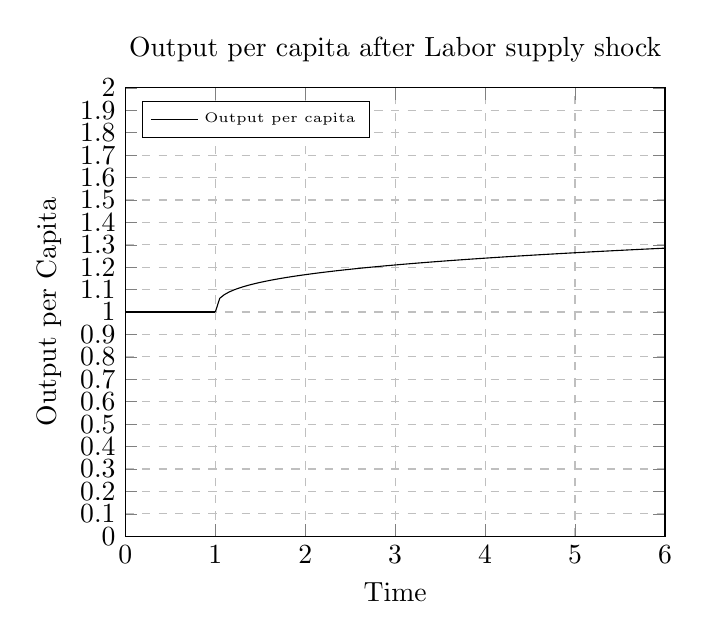
\begin{tikzpicture}
        \begin{axis}[
            title = {Output per capita after Labor supply shock},
            ylabel = {Output per Capita},
            xlabel = {Time},
            xmin = 0, xmax = 6,
            ymin = 0, ymax = 2,
            xtick = {0,1,2,3,4,5,6},
            ytick = {0,0.1,0.2,0.3,0.4,0.5,0.6,0.7,0.8,0.9,1.0,1.1,1.2,1.3,1.4,1.5,1.6,1.7,1.8,1.9,2.0},
            legend pos = north west,
            xmajorgrids = true, ymajorgrids = true, grid style = dashed,
          ]
          \draw (axis cs:0,1) -- (axis cs: 1,1);
          \addplot[domain = 1:6,color = black,samples = 100]{(1/6) * ((x-1)^(1/3)) + 1};
          \addlegendentry{\tiny Output per capita}
        \end{axis}
      \end{tikzpicture}
    \end{center}
  \end{tcolorbox}
\end{solution}
\begin{problem}{True/False}
  \begin{enumerate}[(a)]
    \item According to the Solow growth model, an earthquake that destroys a large fraction of a country's capital stock will cause a decline in the steady state level of output.
    \item According to the Principle of Transition Dynamics, the further below an economy is from its steady state, the faster it will grow.
  \end{enumerate}
\end{problem}
\begin{solution}
  \begin{tcolorbox}[colback = white, title = (a)]
    This is \textbf{false}, because (assuming all else equal), an earthquake has no effect on the investment rate or the depreciation rate, meaning there is no difference in the steady state level of output.
  \end{tcolorbox}
  \begin{tcolorbox}[colback = white, title = (b)]
    This is \textbf{true}, because the further below steady state an economy is, the marginal product of capital is far higher than depreciation, so output will rise while depreciation catches up to marginal product of capital, by which the rate of output growth will start falling as it approaches steady state.
  \end{tcolorbox}
\end{solution}
\end{document}
